\documentclass[11pt]{article}

\usepackage[letterpaper,margin=0.78in,headheight=15pt]{geometry}
\usepackage[T1]{fontenc}
\usepackage[utf8]{inputenc}
\usepackage{lmodern}
\usepackage{microtype}
\usepackage{amsmath,amssymb,amsthm,mathtools,bm}
\usepackage{booktabs,tabularx,array,longtable,multirow}
\usepackage{enumitem}
\usepackage{xcolor}
\usepackage{graphicx}
\usepackage{caption}
\usepackage{subcaption}
\usepackage{float}
\usepackage{tikz}
\usetikzlibrary{arrows.meta,positioning,calc,fit,backgrounds,decorations.pathreplacing,shapes.geometric}
\usepackage{pgfplots}
\pgfplotsset{compat=1.18}
\usepackage[most]{tcolorbox}
\usepackage{listings}
\usepackage{fancyhdr}
\usepackage{titlesec}
\usepackage{hyperref}
\usepackage[nameinlink,noabbrev]{cleveref}
\usepackage{xurl}

\definecolor{ink}{HTML}{18222D}
\definecolor{slate}{HTML}{4D5B6A}
\definecolor{violet}{HTML}{6D5BD0}
\definecolor{violetdark}{HTML}{4E3DA8}
\definecolor{teal}{HTML}{0C7C86}
\definecolor{bluegray}{HTML}{EAF0F5}
\definecolor{lavender}{HTML}{F0EDFF}
\definecolor{mint}{HTML}{E9F7F4}
\definecolor{amber}{HTML}{A86500}
\definecolor{amberbg}{HTML}{FFF5DD}
\definecolor{redish}{HTML}{A43842}
\definecolor{redbg}{HTML}{FFF0F1}
\definecolor{greenish}{HTML}{277A55}
\definecolor{greenbg}{HTML}{EAF7F0}

\hypersetup{
  colorlinks=true,
  linkcolor=violetdark,
  citecolor=teal,
  urlcolor=teal,
  pdftitle={When the Jacobian Lens Meets Curvature: Gemma 4 31B as a Case Study},
  pdfauthor={Course handout prepared for Karl Burtram},
  pdfsubject={Theoretical deep learning, mechanistic interpretability, Jacobian lenses, local linearity}
}

\pagestyle{fancy}
\fancyhf{}
\lhead{Theoretical Deep Learning Case Study}
\rhead{Gemma 4 and Nonlinear Transport}
\cfoot{\thepage}
\renewcommand{\headrulewidth}{0.4pt}

\titleformat{\section}{\Large\bfseries\color{ink}}{\thesection}{0.7em}{}
\titleformat{\subsection}{\large\bfseries\color{violetdark}}{\thesubsection}{0.65em}{}
\titleformat{\subsubsection}{\normalsize\bfseries\color{teal}}{\thesubsubsection}{0.55em}{}

\setlist[itemize]{topsep=3pt,itemsep=2pt,parsep=1pt,leftmargin=1.45em}
\setlist[enumerate]{topsep=3pt,itemsep=2pt,parsep=1pt,leftmargin=1.65em}
\setlength{\parindent}{0pt}
\setlength{\parskip}{5.5pt}
\setlength{\emergencystretch}{2em}

\newcommand{\R}{\mathbb{R}}
\newcommand{\E}{\mathbb{E}}
\newcommand{\Var}{\operatorname{Var}}
\newcommand{\Cov}{\operatorname{Cov}}
\newcommand{\diag}{\operatorname{diag}}
\newcommand{\softmax}{\operatorname{softmax}}
\newcommand{\rank}{\operatorname{rank}}
\newcommand{\supp}{\operatorname{supp}}
\newcommand{\Jbar}{\overline{J}}
\newcommand{\Norm}[1]{\left\lVert #1 \right\rVert}
\newcommand{\Abs}[1]{\left\lvert #1 \right\rvert}
\newcommand{\ip}[2]{\left\langle #1,#2 \right\rangle}
\newcommand{\dd}{\,\mathrm{d}}
\newcommand{\cO}{\mathcal{O}}
\newcommand{\eps}{\varepsilon}
\newcommand{\given}{\,\middle|\,}
\newcommand{\eid}[1]{{\footnotesize\texttt{[#1]}}}

\newtheorem{proposition}{Proposition}
\newtheorem{lemma}{Lemma}
\theoremstyle{definition}
\newtheorem{definition}{Definition}
\theoremstyle{remark}
\newtheorem{remark}{Remark}

\newtcolorbox{takeawaybox}[1][]{
  enhanced, breakable, colback=lavender, colframe=violet,
  boxrule=0.8pt, arc=2mm, left=2.5mm,right=2.5mm,top=1.8mm,bottom=1.8mm,
  fonttitle=\bfseries, title={Key takeaway}, #1
}
\newtcolorbox{statusbox}[1][]{
  enhanced, breakable, colback=bluegray, colframe=slate,
  boxrule=0.7pt, arc=2mm, left=2.5mm,right=2.5mm,top=1.8mm,bottom=1.8mm,
  fonttitle=\bfseries, title={Evidence status}, #1
}
\newtcolorbox{pitfallbox}[1][]{
  enhanced, breakable, colback=amberbg, colframe=amber,
  boxrule=0.7pt, arc=2mm, left=2.5mm,right=2.5mm,top=1.8mm,bottom=1.8mm,
  fonttitle=\bfseries, title={Common pitfall}, #1
}
\newtcolorbox{resultbox}[1][]{
  enhanced, breakable, colback=greenbg, colframe=greenish,
  boxrule=0.7pt, arc=2mm, left=2.5mm,right=2.5mm,top=1.8mm,bottom=1.8mm,
  fonttitle=\bfseries, title={Interpretation}, #1
}
\newtcolorbox{warningbox}[1][]{
  enhanced, breakable, colback=redbg, colframe=redish,
  boxrule=0.7pt, arc=2mm, left=2.5mm,right=2.5mm,top=1.8mm,bottom=1.8mm,
  fonttitle=\bfseries, title={Validity warning}, #1
}

\lstdefinestyle{code}{
  basicstyle=\ttfamily\small,
  backgroundcolor=\color{bluegray},
  frame=single,
  rulecolor=\color{slate!50},
  keywordstyle=\bfseries\color{violetdark},
  commentstyle=\itshape\color{slate},
  stringstyle=\color{teal},
  showstringspaces=false,
  breaklines=true,
  columns=fullflexible,
  xleftmargin=0.5em,
  xrightmargin=0.5em,
  aboveskip=6pt,
  belowskip=6pt
}
\lstset{style=code}

\graphicspath{{./}{figures/}{/mnt/data/}}

\begin{document}
\pagenumbering{gobble}

\begin{titlepage}
\thispagestyle{empty}
\vspace*{0.7in}

{\color{violetdark}\rule{\textwidth}{2.2pt}}
\vspace{0.35in}

{\Huge\bfseries\color{ink} When the Jacobian Lens Meets Curvature\par}
\vspace{0.16in}
{\LARGE\bfseries\color{violetdark} Gemma 4 31B as a Case Study in the Limits of Linear Transport\par}

\vspace{0.42in}
{\large A graduate-level handout for theoretical deep learning and mechanistic interpretability\par}

\vspace{0.55in}
\begin{tcolorbox}[enhanced,colback=lavender,colframe=violet,boxrule=1pt,arc=2mm,left=4mm,right=4mm,top=3mm,bottom=3mm]
\textbf{Central question.} A transformer is a composition of nonlinear attention, normalization, and gated-MLP blocks. Why can a single linear map between a middle layer and the output ever work, and what should we conclude when it fails on Gemma 4 31B?
\end{tcolorbox}

\vfill
\begin{tabular}{@{}ll@{}}
Prepared for: & Karl Burtram \quad (graduate computer science course example)\\
Source case study: & J-space Part 2 pilot and accompanying technical exchange\\
Version: & August 2026 (Study-2 calibrated terminal state; evidence \texttt{gm2-backend-parity-calibration-v1}, \texttt{gm2-stage1-relicense-v1})\\
\end{tabular}

\vspace{0.25in}
{\small\color{slate}
This handout separates three layers of claims: published J-lens methodology, official Gemma 4 architecture facts, and checkpoint-specific pilot measurements supplied with the course materials. The pilot findings are treated as provisional until the final autograd-JVP validation is complete.}

\vspace{0.25in}
{\color{violetdark}\rule{\textwidth}{2.2pt}}
\end{titlepage}

\pagenumbering{roman}
\tableofcontents
\clearpage
\pagenumbering{arabic}

\section*{Learning objectives}
\addcontentsline{toc}{section}{Learning objectives}
After working through this handout, a student should be able to:
\begin{enumerate}
  \item derive the Jacobian-lens transport map and state the assumptions hidden inside the phrase ``locally linear'';
  \item distinguish differentiability, finite-radius linearity, and cross-context stability;
  \item derive curvature diagnostics from Taylor expansion, including homogeneity, odd-symmetry, and additivity tests;
  \item identify where RMSNorm, gated MLPs, and softmax attention generate first- and second-order effects;
  \item interpret the Gemma 4 31B pilot without overclaiming either ``no workspace'' or ``calculus failure'';
  \item design a model-family preflight gate that separates numerical floors, true curvature, and mean-Jacobian cancellation;
  \item evaluate nonlinear recovery strategies and explain why successful decoding is not automatically a causal intervention license.
\end{enumerate}

\begin{takeawaybox}
The surprise is \emph{not} that a 60-layer transformer is globally nonlinear. The surprise is that, at the finite intervention scales needed by the J-space assay, Gemma 4 31B appears not to admit a useful fixed linear transport map through the middle band where the original workspace paper looks. The appropriate conclusion is instrument-specific: the mid-band J-lens is not yet licensed on this checkpoint.
\end{takeawaybox}

\section{The case in one page}

\subsection{What the supplied pilot reports}
The supplied campaign materials report the following checkpoint-specific pattern for \texttt{gemma-4-31B-it}:
\begin{itemize}
  \item The answer token is almost unreadable in the final output basis from approximately layer 2 through layer 40. Its median rank remains in the tens of thousands, then collapses sharply around layers 42--44 and reaches rank 1 by approximately layer 52.
  \item The original paper's relative workspace band, 37--62\% of depth, corresponds to layers 22--37 in a 60-layer model and lies entirely inside this opaque region.
  \item A vanilla logit lens and a small Jacobian-based readout both fail in this band, so simple output-coordinate mismatch is not repaired by the tested linear transport.
  \item In the later nonlinear-transport harness, the same code gives near-ideal doubling ratios of roughly 1.98--2.02 on an OLMo control, while Gemma's response becomes less linear as perturbation scale grows. One reported layer-37 ratio falls from about 1.27 to 0.87, while normalized additivity error grows from about 0.76 to 1.30.
  \item Multiple corpus slices produce strongly differing estimated Jacobians, suggesting that an average map may cancel context-specific tangent planes.
\end{itemize}

\begin{statusbox}
The strongest current interpretation is a combination of two possible failures:
\begin{enumerate}
  \item \textbf{within-context curvature}: even the prompt-specific tangent does not predict finite ablation-size moves; and/or
  \item \textbf{between-context heterogeneity}: prompt-specific tangents may be valid locally but do not average to a useful fixed map.
\end{enumerate}
The gold-standard closing experiment is an exact autograd Jacobian-vector product (JVP) compared with finite differences over a carefully delivered $\eps$ ladder in fp32.
\emph{Update (2026-08-02): that experiment ran in the isolated
\texttt{jspace\_gemma} track and stopped at its own precommitted
cross-backend consistency gate --- see \cref{sec:autopsy-ran}. At that
date the track's classification was a \textbf{methods blocker}.}
\emph{Update (2026-08-03, Study 2): a separately preregistered,
target-blind backend calibration (G2.1) froze a pooled mixed-precision
exact-backend ceiling of $0.07870368901355948$
($=\max(3\cdot q99_{\mathrm{disagreement}}, q99_{\mathrm{ten\ quanta}})$,
route \texttt{benign\_scheduling\_floor}); the preserved Study-1
all-slot discrepancy ($0.002458111383020878$) lies within it and the
selected scientific slot is bit-identical, so G2.2 mechanically
relicensed the unchanged five-layer \texttt{local\_tangent\_mismatch}
classifier (L22/L30/L37/L44/L52) as a \textbf{closed exact-JVP
finite-scale methods result} over the tested prompts, layers,
directions, target map, and doses
[\texttt{gm2-backend-parity-calibration-v1},
\texttt{gm2-stage1-relicense-v1}]. Study 1's failed $10^{-5}$ gate
remains immutable history; it is not retroactively passed. The result
still licenses no nondifferentiability, named-mechanism,
missing-information, or workspace conclusion.}
\end{statusbox}

\subsection{What the result does not establish}
It does \emph{not} establish any of the following:
\begin{itemize}
  \item that Gemma 4 is ``non-differentiable'' or incompatible with backpropagation;
  \item that no concept analogous to a workspace exists in Gemma;
  \item that every Gemma 4 size or checkpoint has the same geometry;
  \item that the abrupt late readout transition is itself proof of nonlinearity;
  \item that a nonlinear probe could not decode the mid-layer state;
  \item that the original J-lens results are invalid on the models for which the transport premise passes empirical checks.
\end{itemize}

\begin{pitfallbox}
``The logit lens cannot read the state'' and ``the downstream map is nonlinear'' are different statements. A fixed linear rotation can make an intermediate state opaque to the unembedding while remaining perfectly linear. Nonlinearity requires a response test, not merely a bad token ranking.
\end{pitfallbox}

\section{From residual stream to Jacobian lens}

\subsection{A context-indexed downstream map}
Let $x$ denote a prompt and its clean forward-pass state. At layer $\ell$ and source position $t$, the residual vector is
\[
  h_{\ell,t}(x) \in \R^d.
\]
For a target position $t'\ge t$, define the downstream map
\[
  F_{x,\ell,t\rightarrow t'}: \R^d \rightarrow \R^d
\]
by replacing the clean source activation with an arbitrary vector $z$ and running the rest of the model:
\[
  F_{x,\ell,t\rightarrow t'}(z)
  := h_{L,t'}\bigl(x; h_{\ell,t}\leftarrow z\bigr).
\]
The causal response to an additive intervention $\delta$ is
\begin{equation}
  \Delta_x(\delta)
  := F_x(h+\delta)-F_x(h),
  \qquad h=h_{\ell,t}(x),
  \label{eq:delta}
\end{equation}
where indices are suppressed for readability.

The prompt-specific Jacobian is
\begin{equation}
  J_x := D F_x(h)
  = \left.\frac{\partial F_x(z)}{\partial z}\right|_{z=h}
  \in \R^{d\times d}.
  \label{eq:promptJ}
\end{equation}
For an infinitesimal perturbation, $J_x\delta$ is the exact first-order response.

\subsection{The corpus-averaged transport map}
The J-lens paper averages over prompts, source positions, and current-or-future target positions:
\begin{equation}
  \Jbar_\ell
  = \E_{x,t,t'\ge t}\left[
    \frac{\partial h_{L,t'}}{\partial h_{\ell,t}}
  \right].
  \label{eq:meanJ}
\end{equation}
This produces one context-independent $d\times d$ matrix per layer. Its purpose is not to reconstruct one prompt exactly. It is intended to represent a typical causal disposition of a direction in the residual stream.

Let $N_f$ be the final normalization and $W_U\in\R^{V\times d}$ the unembedding. The paper's readout is
\begin{equation}
  \operatorname{lens}_\ell(h)
  = \softmax\!\left(W_U N_f(\Jbar_\ell h)\right).
  \label{eq:lens}
\end{equation}
For Gemma 4 31B, the language-model head is tied to the token embedding matrix. A final elementwise softcap is then applied to logits:
\begin{equation}
  s_c(z)_i = c\tanh(z_i/c),
  \qquad c=30.
  \label{eq:softcap}
\end{equation}
Because $s_c$ is strictly increasing, it does not change token ranks, although it does change logit differences and derivatives.

\subsection{Token directions and the J-space}
Ignoring the final normalization for a moment, the score of token $w$ is
\[
  u_w^\top \Jbar_\ell h,
\]
where $u_w^\top$ is row $w$ of $W_U$. Thus a corresponding source-layer direction is
\begin{equation}
  d_{\ell,w} = \Jbar_\ell^\top u_w.
  \label{eq:token_direction}
\end{equation}
The paper often describes these through the rows of $W_U\Jbar_\ell$; 
\cref{eq:token_direction} is the equivalent column-vector convention.

Collect normalized token directions as columns of $D_\ell\in\R^{d\times V}$. For sparsity budget $k$, an idealized J-space is the union of nonnegative sparse cones
\begin{equation}
  \mathcal{J}_{\ell,k}
  = \left\{D_\ell\alpha:
      \alpha\ge 0,\; \Norm{\alpha}_0\le k\right\}.
  \label{eq:jspace}
\end{equation}
Since $V>d$, the dictionary is overcomplete. Sparse nonnegative decomposition supplies a practical coordinate system, not a unique linear basis.

\subsection{A subtle point: a Jacobian predicts differences, not absolute states}
Taylor's theorem around the clean state $h$ gives
\begin{equation}
  F_x(h+\delta)
  \approx F_x(h)+J_x\delta.
  \label{eq:affine_taylor}
\end{equation}
This is an \emph{affine} approximation. By contrast, the lens applies $\Jbar_\ell h$ without an intercept. Therefore the readout makes an additional empirical move: it treats the activation vector itself as a causal direction from a chosen origin, then asks what output tendency that direction would have on average.

This distinction is not necessarily fatal. Final RMS normalization removes much of the scale information, and residual-stream representations are often interpreted directionally. But it means that two properties should be tested separately:
\begin{enumerate}
  \item Does $J_x\delta$ predict the response to the actual interventions used by the experiment?
  \item Does $\Jbar_\ell h$ provide a useful vocabulary coordinate system for clean activations?
\end{enumerate}
A lens may decode usefully without reconstructing the final state, and a tangent may predict tiny perturbations without supporting finite projection ablations.

\section{Three different meanings of ``linear''}

\subsection{Differentiability}
A function is differentiable at $h$ if there exists a linear map $J$ such that
\[
  \lim_{\Norm{\delta}\to 0}
  \frac{\Norm{F(h+\delta)-F(h)-J\delta}}{\Norm{\delta}}=0.
\]
This is the requirement used by backpropagation. It is infinitesimal and pointwise.

\subsection{Finite-radius local linearity}
An intervention study needs more. For a non-negligible radius $r$, it needs
\begin{equation}
  F(h+\delta)-F(h)\approx J\delta
  \qquad \text{for }\Norm{\delta}\le r
  \label{eq:finite_radius}
\end{equation}
for directions and magnitudes resembling the intervention. A projection that removes 10--20\% of residual energy is not infinitesimal merely because the model is differentiable.

\begin{proposition}[Taylor remainder bound]
Suppose $F:\R^d\to\R^m$ is twice continuously differentiable on the line segment from $h$ to $h+\delta$, and
\[
  \sup_{s\in[0,1]}\Norm{D^2F(h+s\delta)}_{\mathrm{op}}\le M.
\]
Then
\begin{equation}
  \Norm{F(h+\delta)-F(h)-DF(h)\delta}
  \le \frac{M}{2}\Norm{\delta}^2.
  \label{eq:taylor_bound}
\end{equation}
\end{proposition}

\begin{proof}
Use the integral form of Taylor's theorem:
\[
F(h+\delta)-F(h)-DF(h)\delta
=\int_0^1(1-s)D^2F(h+s\delta)[\delta,\delta]\dd s.
\]
Taking norms yields \cref{eq:taylor_bound}.
\end{proof}

If $\Norm{DF(h)v}\ge m$ for a unit direction $v$, the relative tangent error for $\delta=\eps v$ is bounded by approximately $M\eps/(2m)$. Thus relative error generally grows linearly with perturbation radius, even though absolute remainder grows quadratically.

\subsection{Cross-context stability}
The J-lens requires a third property. Let $J_x$ be the prompt-specific tangent and $\Jbar=\E[J_x]$. A fixed lens is useful only if $J_x$ does not vary so much that averaging destroys the signal.

Write
\begin{equation}
  \Delta_x(\delta)=J_x\delta+r_x(\delta),
  \qquad r_x(\delta)=\cO(\Norm{\delta}^2).
  \label{eq:context_decomp}
\end{equation}
Then
\begin{equation}
  \Delta_x(\delta)-\Jbar\delta
  = (J_x-\Jbar)\delta+r_x(\delta).
  \label{eq:mean_error_decomp}
\end{equation}
The first term is \emph{tangent heterogeneity}; the second is \emph{within-context curvature}.

\begin{proposition}[Mean-map error decomposition]
For a fixed $\delta$,
\begin{align}
  \E\Norm{\Delta_x(\delta)-\Jbar\delta}^2
  &= \E\Norm{(J_x-\Jbar)\delta}^2
  + \E\Norm{r_x(\delta)}^2 \\
  &\quad +2\E\ip{(J_x-\Jbar)\delta}{r_x(\delta)}.
  \label{eq:mse_decomp}
\end{align}
\end{proposition}

At sufficiently small $\eps$, the heterogeneity term scales as $\eps^2$ in squared error, while the curvature term scales as $\eps^4$. In relative error, context heterogeneity can produce a nonzero floor as $\eps\to0$, whereas smooth curvature tends to vanish with $\eps$. This scaling law is the cleanest theoretical way to separate the two.

\begin{takeawaybox}
Backpropagation needs only differentiability at the current point. A J-space causal assay needs a much stronger package: useful finite-radius linearity along intervention directions, plus enough cross-context stability that one averaged tangent remains meaningful.
\end{takeawaybox}

\section{Why residual transformers can look linear, and why they need not}

\subsection{Residual composition}
A simplified residual block has the form
\begin{equation}
  B_k(h)=h+f_k(h).
\end{equation}
Its Jacobian is
\begin{equation}
  DB_k(h)=I+Df_k(h).
\end{equation}
For a stack $F=B_{L-1}\circ\cdots\circ B_\ell$,
\begin{equation}
  DF(h_\ell)=\prod_{k=\ell}^{L-1}\left(I+Df_k(h_k)\right),
  \label{eq:residual_product}
\end{equation}
with factors ordered along the forward pass. The identity path prevents a perturbation from being multiplied only through nonlinear branches. This often makes local transport better conditioned than in a plain feed-forward chain.

However, the skip connection does not remove curvature. Differentiating once more produces sums of Hessian terms transported through all downstream Jacobians. A few strongly curved or context-sensitive blocks can dominate the composite remainder.

\subsection{The Gemma 4 text block}
For the dense 31B checkpoint, the implementation follows the schematic
\begin{align}
  a &= h + N^{\mathrm{post}}_{A}\!\left(
      A\left(N^{\mathrm{pre}}_{A}(h)\right)\right),
  \label{eq:gemma_attn_block}\\
  h^+ &= a + N^{\mathrm{post}}_{M}\!\left(
      M\left(N^{\mathrm{pre}}_{M}(a)\right)\right).
  \label{eq:gemma_mlp_block}
\end{align}
There is an RMSNorm before and after each attention or MLP branch. Q and K are also RMS-normalized inside attention.

\begin{figure}[H]
\centering
\resizebox{\textwidth}{!}{%
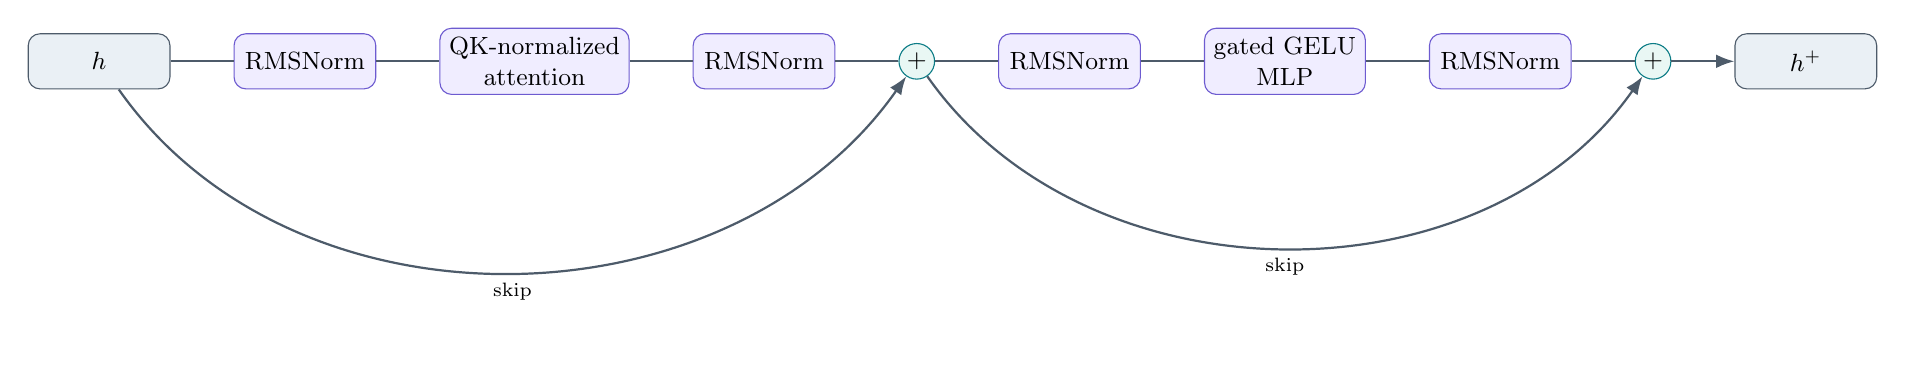
\begin{tikzpicture}[
  node distance=7mm and 8mm,
  box/.style={draw=slate,rounded corners=1.5mm,fill=bluegray,minimum height=7mm,minimum width=18mm,align=center,font=\small},
  nonlin/.style={draw=violet,rounded corners=1.5mm,fill=lavender,minimum height=7mm,minimum width=18mm,align=center,font=\small},
  sum/.style={circle,draw=teal,fill=mint,inner sep=1.2pt,font=\small\bfseries},
  arr/.style={-Latex,thick,draw=slate}
]
\node[box] (h) {$h$};
\node[nonlin,right=of h] (n1) {RMSNorm};
\node[nonlin,right=of n1] (attn) {QK-normalized\\attention};
\node[nonlin,right=of attn] (n2) {RMSNorm};
\node[sum,right=of n2] (s1) {$+$};
\node[nonlin,right=of s1] (n3) {RMSNorm};
\node[nonlin,right=of n3] (mlp) {gated GELU\\MLP};
\node[nonlin,right=of mlp] (n4) {RMSNorm};
\node[sum,right=of n4] (s2) {$+$};
\node[box,right=of s2] (out) {$h^+$};
\draw[arr] (h)--(n1)--(attn)--(n2)--(s1)--(n3)--(mlp)--(n4)--(s2)--(out);
\draw[arr] (h) to[out=-55,in=-125] node[below,font=\scriptsize] {skip} (s1);
\draw[arr] (s1) to[out=-55,in=-125] node[below,font=\scriptsize] {skip} (s2);
\end{tikzpicture}%
}
\caption{A dense Gemma 4 text block. Residual paths carry perturbations directly, while normalization, attention routing, and the gated MLP create state-dependent Jacobians and curvature.}
\label{fig:gemma_block}
\end{figure}

\subsection{RMSNorm is smooth but curved}
Ignoring learned scale for a moment, define
\begin{equation}
  r(h)=\sqrt{\frac{1}{d}\Norm{h}^2+\epsilon_0},
  \qquad N(h)=\gamma\odot\frac{h}{r(h)}.
\end{equation}
Its directional derivative is
\begin{equation}
  DN(h)[u]
  =\gamma\odot\left(
      \frac{u}{r}
      -\frac{h\,\ip{h}{u}}{d\,r^3}
    \right).
  \label{eq:rmsnorm_jac}
\end{equation}
The second derivative is
\begin{align}
  D^2N(h)[u,v]
  =\gamma\odot\Bigg(&
   -\frac{u\,\ip{h}{v}+v\,\ip{h}{u}+h\,\ip{u}{v}}{d\,r^3}
   \nonumber\\
   &+\frac{3h\,\ip{h}{u}\ip{h}{v}}{d^2r^5}
  \Bigg).
  \label{eq:rmsnorm_hess}
\end{align}
Thus RMSNorm is differentiable, but radial and tangential perturbations are transformed differently. Repeating pre- and post-normalization twice per block gives many opportunities for state-dependent gain and direction changes.

\subsection{A gated MLP has multiplicative curvature}
Gemma's dense MLP has the form
\begin{equation}
  M(x)=W_d\left(\phi(W_gx)\odot W_ux\right),
  \label{eq:gated_mlp}
\end{equation}
where $\phi$ is a tanh-approximated GELU. Let $g=W_gx$ and $u=W_ux$. For perturbation $\delta$,
\begin{align}
  DM(x)[\delta]
  =W_d\Big(&
    \phi'(g)\odot(W_g\delta)\odot u
    +\phi(g)\odot(W_u\delta)
  \Big).
  \label{eq:mlp_jac}
\end{align}
For two directions $\delta_1,\delta_2$,
\begin{align}
D^2M(x)[\delta_1,\delta_2]
=W_d\Big(&
 \phi''(g)\odot(W_g\delta_1)\odot(W_g\delta_2)\odot u
 \nonumber\\
 &+\phi'(g)\odot(W_g\delta_1)\odot(W_u\delta_2)
 \nonumber\\
 &+\phi'(g)\odot(W_g\delta_2)\odot(W_u\delta_1)
\Big).
\label{eq:mlp_hess}
\end{align}
The elementwise product is important. Even if $\phi$ were nearly linear, the gate and value branches multiply, creating cross terms.

\subsection{Attention is a context-dependent router}
For one query, write
\begin{equation}
  a=\softmax(z),\qquad z=\frac{qK^\top}{\tau},\qquad y=aV.
\end{equation}
The softmax derivative is
\begin{equation}
  Da(z)[\eta]
  =S(a)\eta,
  \qquad S(a)=\diag(a)-aa^\top.
  \label{eq:softmax_jac}
\end{equation}
A perturbation to the residual stream can change $q$, $K$, and $V$ simultaneously. Consequently, attention's Jacobian contains a value-path term and routing terms. Its Hessian includes:
\begin{itemize}
  \item derivatives of $S(a)$, which change when the attention distribution changes;
  \item bilinear $qK^\top$ cross terms;
  \item derivatives introduced by QKNorm;
  \item sequence-level effects, because moving one source token can alter routes to many targets.
\end{itemize}
A fixed attention pattern makes the value aggregation linear in $V$. The full attention block is not fixed-pattern, and finite perturbations can move mass between competing routes.

\subsection{A small routing toy model}
Consider
\begin{equation}
  F(h)=h+v\,\sigma(q^\top h),
  \label{eq:routing_toy}
\end{equation}
where $\sigma$ is the logistic sigmoid. This is a one-route caricature of attention. Its Jacobian is
\begin{equation}
  DF(h)=I+v\,\sigma(q^\top h)(1-\sigma(q^\top h))q^\top,
\end{equation}
and its Hessian is proportional to
\begin{equation}
  v\,\sigma(1-\sigma)(1-2\sigma)\,q\otimes q.
\end{equation}
Two prompts with different $q^\top h$ have different tangent maps. A finite perturbation that moves $q^\top h$ across a routing transition is poorly approximated by one tangent, even though the function is smooth everywhere.

\section{A mathematical preflight for linear transport}

\subsection{The response object}
Fix a clean state $h$, a unit direction $v$, and a scale $\eps$. Define
\begin{equation}
  \Delta(\eps;v)=F(h+\eps v)-F(h).
\end{equation}
The ideal first-order model is $\eps Jv$.

\subsection{Tangent accuracy}
Given an exact autograd JVP $j=Jv$, define
\begin{align}
  e_{\mathrm{tan}}(\eps;v)
  &=\frac{\Norm{\Delta(\eps;v)-\eps j}}
          {\Norm{\Delta(\eps;v)}+\eta},
  \label{eq:tangent_error}\\
  c_{\mathrm{tan}}(\eps;v)
  &=\frac{\ip{\Delta(\eps;v)}{j}}
          {\Norm{\Delta(\eps;v)}\Norm{j}+\eta},
  \label{eq:tangent_cos}\\
  g_{\mathrm{tan}}(\eps;v)
  &=\frac{\Norm{\Delta(\eps;v)}}{\eps\Norm{j}+\eta}.
  \label{eq:tangent_gain}
\end{align}
A useful tangent has small relative error, cosine near 1, and gain near 1 over the actual intervention range.

\subsection{Homogeneity and the doubling test}
For a linear map, $\Delta(2\eps;v)=2\Delta(\eps;v)$. Define the vector defect
\begin{equation}
  e_{\mathrm{hom}}(\eps;v)
  =\frac{\Norm{\Delta(2\eps;v)-2\Delta(\eps;v)}}
  {2\Norm{\Delta(\eps;v)}+\eta}.
  \label{eq:hom_defect}
\end{equation}
Under a second-order Taylor expansion,
\begin{equation}
  \Delta(2\eps;v)-2\Delta(\eps;v)
  =\eps^2 D^2F(h)[v,v]+\cO(\eps^3).
\end{equation}
A scalar norm ratio
\begin{equation}
  \rho_2(\eps;v)
  =\frac{\Norm{\Delta(2\eps;v)}}{\Norm{\Delta(\eps;v)}}
\end{equation}
should equal 2, but it is insufficient by itself because the response could rotate while preserving its norm. Report both ratio and vector defect.

\subsection{Odd symmetry estimates directional curvature}
The centered second difference is
\begin{equation}
  C_{\pm}(\eps;v)
  :=\Delta(\eps;v)+\Delta(-\eps;v)
  =\eps^2D^2F(h)[v,v]+\cO(\eps^4).
  \label{eq:odd_sym}
\end{equation}
A normalized curvature score is
\begin{equation}
  e_{\pm}(\eps;v)
  =\frac{\Norm{\Delta(\eps;v)+\Delta(-\eps;v)}}
  {\Norm{\Delta(\eps;v)-\Delta(-\eps;v)}+\eta}.
\end{equation}
This is especially useful because it does not require an explicitly materialized Jacobian.

\subsection{Superposition and cross-curvature}
For two directions $v,w$, define the additivity defect
\begin{equation}
  A(\eps;v,w)
  =\Delta(\eps;v+w)-\Delta(\eps;v)-\Delta(\eps;w).
  \label{eq:additivity}
\end{equation}
Taylor expansion gives
\begin{equation}
  A(\eps;v,w)
  =\eps^2D^2F(h)[v,w]+\cO(\eps^3).
  \label{eq:additivity_hess}
\end{equation}
This directly probes whether two concept directions interact under downstream transport.

\subsection{Context stability}
For prompt-specific Jacobians $J_1,\ldots,J_n$, useful diagnostics include
\begin{align}
  \kappa_F &= \frac{\Norm{\frac{1}{n}\sum_i J_i}_F}
  {\frac{1}{n}\sum_i\Norm{J_i}_F},
  \label{eq:cancellation_index}\\
  s_{ij}(v) &= \cos(J_iv,J_jv),
  \label{eq:directional_stability}
\end{align}
plus principal-angle or subspace comparisons for selected output directions. A small $\kappa_F$ means that substantial prompt-specific tangents cancel in the mean.

Full $d\times d$ matrices are not required. One can estimate stability with a shared set of random or intervention-relevant probe directions and JVPs.

\subsection{Layerwise localization}
Let $F_{\ell\rightarrow k}$ map a source intervention at layer $\ell$ to the residual after block $k$. Repeat the diagnostics for every $k>\ell$. If error jumps at a particular block, that block is a mechanistic suspect. If error accumulates gradually, the cause is distributed.

\subsection{The numerical floor in bfloat16}
Bfloat16 has 7 explicit fraction bits. Around a number of order 1, adjacent representable values are separated by roughly $2^{-7}\approx 0.0078$, while unit roundoff is about $2^{-8}\approx 0.0039$. A nominal perturbation can therefore be rounded away or have its direction distorted.

Always record the actually delivered perturbation
\begin{equation}
  \widehat{\delta}=\operatorname{cast}(h+\delta)-h
\end{equation}
and report
\begin{equation}
  f_{\mathrm{norm}}=\frac{\Norm{\widehat{\delta}}}{\Norm{\delta}},
  \qquad
  f_{\mathrm{cos}}=\cos(\widehat{\delta},\delta).
\end{equation}
A curvature claim is invalid if input fidelity is not near 1. Use fp32 injection or a sufficiently large $\eps$ ladder, then confirm that increasing $\eps$ does not merely rescue a precision-limited signal.

\begin{table}[H]
\centering
\small
\caption{A compact transport-gate diagnostic suite.}
\label{tab:diagnostics}
\begin{tabularx}{\textwidth}{@{}p{0.18\textwidth}p{0.28\textwidth}X@{}}
\toprule
\textbf{Test} & \textbf{Linear expectation} & \textbf{What failure suggests}\\
\midrule
Input delivery & $f_{\mathrm{norm}}\approx1$, $f_{\mathrm{cos}}\approx1$ & Numerical floor, hook placement error, dtype conversion, or overwrite\\
Exact JVP & $\Delta(\eps)\approx\eps Jv$ as $\eps\to0$ & Harness mismatch if it fails at tiny faithful $\eps$; curvature if it passes tiny $\eps$ but fails at larger $\eps$\\
Homogeneity & $\Delta(2\eps)=2\Delta(\eps)$ & Directional second-order response\\
Odd symmetry & $\Delta(+\eps)+\Delta(-\eps)\approx0$ & Directional Hessian term\\
Additivity & $\Delta(v+w)=\Delta(v)+\Delta(w)$ & Cross-direction interactions\\
Context stability & $J_xv$ aligns across prompts & Mean-Jacobian cancellation or multiple local charts\\
Layer localization & Error remains low or grows smoothly & A sharp jump identifies a suspect block or architecture transition\\
Positive control & Same harness recovers known linear behavior & Without it, instrument bugs remain live\\
\bottomrule
\end{tabularx}
\end{table}

\section{Gemma 4 31B: architecture facts relevant to transport}

\subsection{Checkpoint anatomy}
The official Gemma 4 report and the released 31B configuration specify the properties in \cref{tab:gemma_arch}.

\begin{table}[H]
\centering
\small
\caption{Selected Gemma 4 31B text architecture properties.}
\label{tab:gemma_arch}
\begin{tabularx}{\textwidth}{@{}p{0.28\textwidth}X@{}}
\toprule
\textbf{Property} & \textbf{Gemma 4 31B text configuration}\\
\midrule
Depth and width & 60 decoder layers; residual width $d=5376$; MLP width 21,504\\
Attention pattern & Five sliding-window layers followed by one full-attention layer, repeated; sliding window 1024\\
Heads & 32 query heads; local head dimension 256; global head dimension 512; 16 local KV heads and 4 global KV heads\\
Normalization & RMSNorm before and after attention; RMSNorm before and after MLP; QKNorm inside attention\\
MLP & Dense gated MLP with tanh-approximated GELU; no MoE block in the 31B checkpoint\\
Global attention & Reuses keys as values in global layers, $V=K$\\
Position encoding & Local RoPE with base $10^4$; proportional partial RoPE for global attention with base $10^6$ and rotary fraction 0.25\\
Vocabulary and head & Vocabulary 262,144; input embedding and unembedding tied\\
Output nonlinearity & Final logit softcap $30\tanh(z/30)$ after the language-model head\\
Per-layer inputs & Disabled for the 31B checkpoint ($\texttt{hidden\_size\_per\_layer\_input}=0$)\\
\bottomrule
\end{tabularx}
\end{table}

\subsection{Architecture audit: the softcap hypothesis needs correction}
An early hypothesis in the supplied exchange was that attention-logit softcapping might squash transport. That mechanism exists in some Gemma-family components and in the Gemma 4 audio encoder, but the official 31B \emph{text} configuration and current implementation do not show a text attention-logit softcap. They do show a \emph{final output-logit} softcap applied after the language-model head.

\begin{warningbox}
The final softcap cannot explain nonlinearity in a residual-to-residual map measured before unembedding. It also cannot explain rank opacity, because an elementwise strictly increasing transform preserves rank. It can affect logit-magnitude linearity, so a logit-space test should either use pre-softcap logits or explicitly include the derivative
\[
  s'_c(z)=\operatorname{sech}^2(z/c).
\]
This is a useful lesson in architecture forensics: verify the exact checkpoint path before assigning a mechanism to a named family feature.
\end{warningbox}

\subsection{Why the local/global pattern is an interesting suspect}
With a 5:1 local-to-global pattern, a perturbation that must influence distant positions can travel through local propagation over several layers or pass through one of only ten full-attention blocks. This can concentrate long-range routing into particular depth locations. It does not prove curvature, but it gives a sharp prediction: layerwise transport error should jump disproportionately at full-attention blocks if routing changes are the cause.

\section{The Gemma pilot as an evidence ladder}

\subsection{Output-basis opacity}
\begin{figure}[H]
\centering
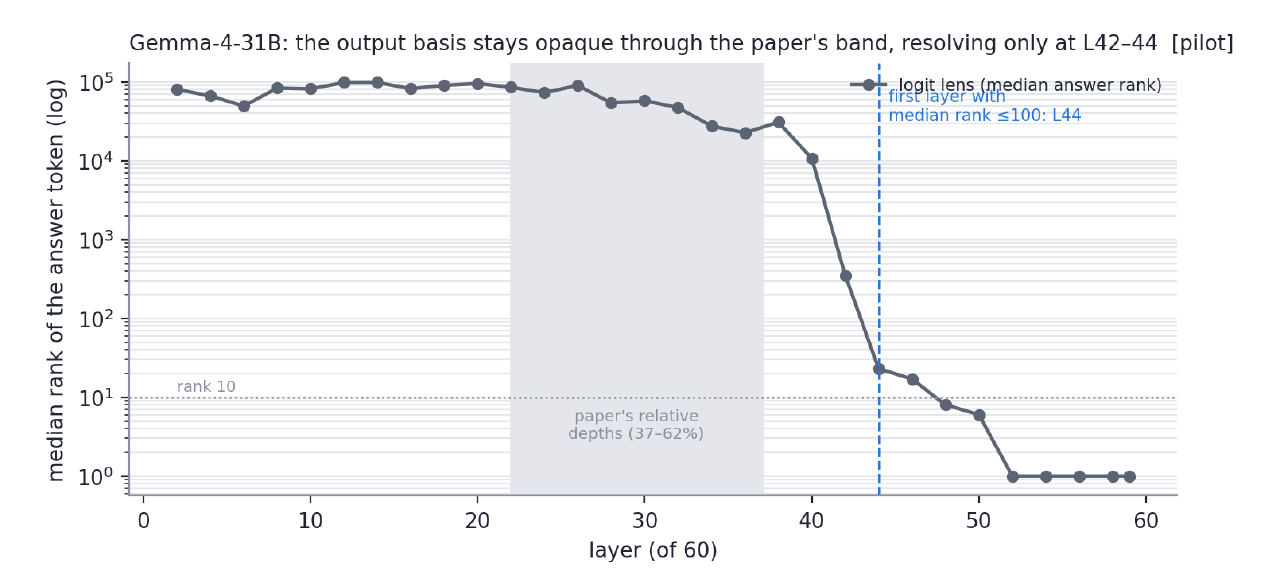
\includegraphics[width=0.96\textwidth]{gemma4_output_basis_pilot.png}
\caption{Pilot result reproduced from the supplied J-space Part 2 handout. The median answer-token rank remains extremely poor through the original paper's middle-layer band, then becomes output-readable around layers 42--44. This chart establishes a late readout transition, not by itself nonlinear transport.}
\label{fig:gemma_rank}
\end{figure}

A linear but rotated representation could produce \cref{fig:gemma_rank}. The surprise becomes stronger only when a fitted or micro-Jacobian transport also fails and finite perturbations violate first-order response tests.

\subsection{The scale trend distinguishes curvature from a precision floor}
Suppose a numerical floor dominates at tiny $\eps$. As $\eps$ increases, delivered perturbations become more faithful and linearity scores should improve. The supplied harness initially found exactly this false-positive signature and corrected it by moving to a faithful scale regime.

The later Gemma pattern reportedly goes in the opposite direction: as $\eps$ grows, the doubling ratio moves farther from 2 and additivity error grows. That is the expected qualitative signature of a Taylor remainder becoming more important.

\subsection{The OLMo positive control}
Under identical code, OLMo reportedly produces doubling ratios near 1.98--2.02 even at perturbations of roughly 10--20\% of residual norm. This does not prove every OLMo direction is linear, but it is a strong positive control: the harness can observe a broad linear regime when one is present.

\subsection{Context-dependent tangents}
The supplied exchange also reports that four disjoint corpus fits at a Gemma middle layer recover strongly differing, nearly orthogonal Jacobian estimates, and that merging them shrinks the map norm. This is the classic geometry of cancellation:
\[
  \Norm{\E[J_x]}_F \ll \E\Norm{J_x}_F.
\]
It supports the between-context term in \cref{eq:mean_error_decomp}. It does not, by itself, establish within-prompt curvature.

\subsection{What is already persuasive, and what remains}
\begin{table}[H]
\centering
\small
\caption{Evidence for and against a real transport failure.}
\begin{tabularx}{\textwidth}{@{}p{0.24\textwidth}X@{}}
\toprule
\textbf{Observation} & \textbf{Inference}\\
\midrule
Input-fidelity gate passes at tested scales & Rules out the simplest bfloat perturbation-loss explanation\\
OLMo passes the same harness & Strong positive control for implementation and metric\\
Gemma worsens as $\eps$ grows & Consistent with curvature, opposite the usual precision-floor trend\\
Within-prompt superposition fails & Evidence that a perfect corpus average would not fully rescue finite-dose interventions\\
Disjoint-corpus Jacobians disagree & Evidence for context-dependent tangent planes and mean-map cancellation\\
Abrupt rank transition at L42--44 & Localizes a late basis conversion, but does not alone prove curvature\\
Exact autograd JVP: ran, then hard-stopped (\cref{sec:autopsy-ran}) & Stage 1 reports \texttt{local\_tangent\_mismatch} at all five layers, but a failed backend-parity gate quarantines the result as diagnostic-only\\
\bottomrule
\end{tabularx}
\end{table}

\begin{resultbox}
A careful present-tense statement is: \emph{Gemma 4 31B appears to violate the fixed, finite-dose linear-transport premise of the middle-band J-lens under the tested setup.} The result is already much more likely to be real than a harness artifact, but the exact JVP ladder is the experiment that should elevate it from a strong pilot to a closed methodological result. \emph{As of 2026-08-02 that ladder had run and did not close the question --- it stopped at a failed cross-backend parity gate (\cref{sec:autopsy-ran}), so the classification at that date was a methods blocker.} \emph{As of 2026-08-03 (Study 2), the target-blind calibrated backend envelope (frozen ceiling $0.07870368901355948$; historical all-slot disagreement $0.002458111383020878$ within it; selected slot bit-identical) closed the question at tested scope: the five-layer \texttt{local\_tangent\_mismatch} classifier is now a closed exact-JVP finite-scale methods result. The measured mismatch (per-layer tangent relative errors $1.36$--$5.36$ at $\eps=0.10$) is 12--52$\times$ the calibrated backend scales; its cause is not identified. For a checkpoint contrast: on the frozen OLMo-3 H6 ladder no in-band cell (L24/L32/L40) is licensed at any tested dose on either mandatory checkpoint, and OLMo-3.1 Think passes only the L56 late anchor at $\eps=0.10$ (12/12; Base 9/12) [\texttt{ol2-transport-validation-joint-v1}]. Transport licensing is model-, checkpoint-, layer-, and dose-specific.}
\end{resultbox}

\section{The autopsy ran: an exact-JVP gate that stopped itself}\label{sec:autopsy-ran}

The closing experiment proposed above executed in August 2026 as an isolated
side track (package \texttt{interpretability/jspace\_gemma}, evidence prefix
\texttt{gm-}, branch merged back after release). Its design followed this
handout's preflight logic exactly: golden-test the instrument, freeze pass
thresholds on a positive control \emph{before} looking at the target, then run
the target once. What happened next is the best available case study in why
those gates exist.

\subsection{The evidence chain}
\begin{enumerate}
  \item \textbf{Goldens} \eid{gm-jvp-goldens-v1}: both PyTorch exact-JVP
  implementations pass analytic and nonlinear tiny-transformer derivative
  checks; finite differences remain labeled secants.
  \item \textbf{OLMo calibration} \eid{gm-jvp-olmo-calibration-v1}: 56 cells /
  1,568 rows on OLMo-3-32B-Think establish the expected shallow-to-late
  faithfulness gradient.
  \item \textbf{Frozen gates} \eid{gm-jvp-olmo-positive-control-v1}: all 14
  target-readiness criteria pass; thresholds (delivery cosine $\ge 0.999$,
  relative-norm error $\le 0.01$, central-tangent relative error $\le 0.1$ at
  declared $\eps = 0.1$, JVP-primal parity $\le 10^{-5}$) are frozen before
  any Gemma number is seen, with recalibration-after-target explicitly
  forbidden.
  \item \textbf{Gemma Stage 1} \eid{gm-jvp-gemma-stage1-v1}: 40 cells / 1,120
  rows at L22/L30/L37/L44/L52, four prompts, four non-lens directions, seven
  relative epsilons 0.0025--0.20.
  \item \textbf{Backend parity} \eid{gm-jvp-gemma-backend-parity-v1}: the
  terminal, failed gate.
\end{enumerate}

\begin{figure}[H]
\centering
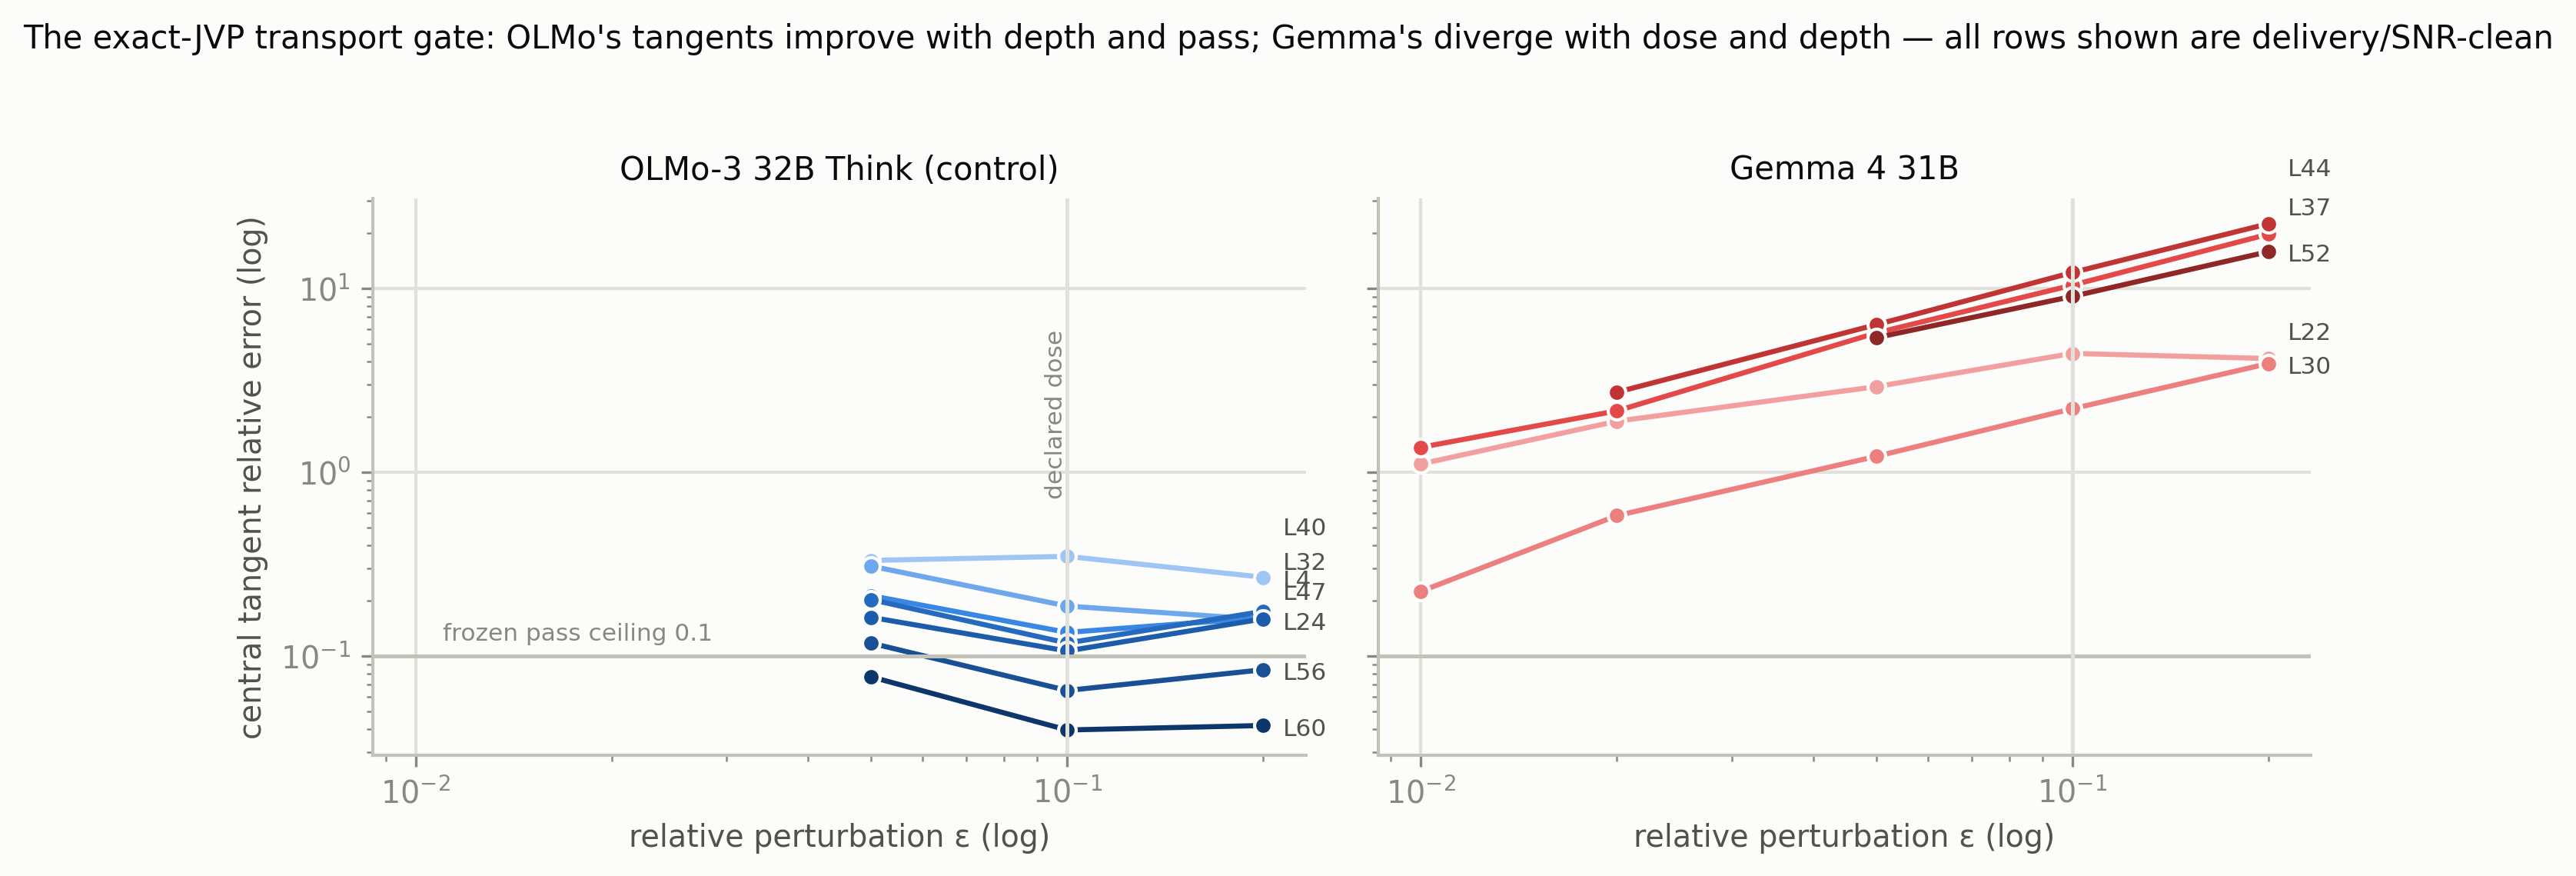
\includegraphics[width=0.98\textwidth]{gmT1_tangent_ladder.png}
\caption{Median central-tangent relative error versus perturbation scale,
delivery- and SNR-clean rows only, from the registered Stage-1 and calibration
row tables. OLMo's error \emph{falls} with depth and sits at or below the
frozen 0.1 ceiling late; Gemma's error is an order of magnitude above the
ceiling at every tested layer and \emph{grows} with $\eps$ --- the Taylor-remainder
signature --- including at L44/L52, inside the band where the output basis
becomes readable. Rows below $\eps \approx 0.05$ (OLMo) / $0.01$ (Gemma) fail
the delivery gate and are correctly absent rather than plotted.
Regenerate: \texttt{scripts/gemma\_transport\_plots.py}.}
\label{fig:gmT1}
\end{figure}

\subsection{Stage 1: operational mismatch at every layer}
Of 1,120 rows, 538 pass delivery, 508 clear measurement SNR 12, and 477 clear
decision SNR 20. All 20 full-forward/suffix checks and all exact-JVP primal
comparisons are bit-exact; the wrong-hook sentinel fires correctly (relative
error 0.3355 against a 0.10 floor). At the declared $\eps = 0.1$ dose, 12/16
primary rows per layer are evaluable and \emph{none pass}; smallest-evaluable
pass counts are 0/12, 0/13, 0/12, 0/13, 1/14 from L22 to L52. The frozen
classifier returns \texttt{local\_tangent\_mismatch} at every layer ---
notably including L44 and L52, which \cref{fig:gemma_rank} might have
suggested were safely inside a late linear-readout regime.

\subsection{The terminal gate: two exact backends, one failed ceiling}
The parity diagnostic replays one registered mismatch row
(\texttt{gm-p001-L52}, Rademacher direction, $\eps=0.05$) under both
\texttt{torch.func.jvp} and \texttt{torch.autograd.functional.jvp}. At the
selected slot the two backends are \emph{bit-identical} and every stored
transport metric replays at zero error --- the mismatch itself is real and
reproducible. But across all eight slots of the original batch, backend
tangent relative error is $0.002458$ against the precommitted $10^{-5}$
ceiling (cosine 0.99999958; maximum absolute difference 0.0390625, a
bf16-scale quantum). One criterion fails; under the plan's hard-stop rule the
track terminates.

\begin{warningbox}
The gate was \emph{not} weakened after seeing the target, and the one
agreeing slot was \emph{not} selected to continue. The licensed sentence is
methods-only: \emph{``On Gemma 4 31B, an exact-JVP transport audit stopped at
a precommitted cross-backend consistency gate: the selected replay agreed
exactly, but the full matched batch exceeded the relative-error tolerance, so
downstream mechanism and workspace interpretation were not licensed.''}
Everything in \cref{fig:gmT1}'s right panel is therefore
\textbf{diagnostic, not mechanism evidence}.
\end{warningbox}

\subsection{What this changes in the claim ledger}
Licensed now (claim ids GM-C01--C05): the instrument passes goldens; the OLMo
control passes the frozen gate in this runtime; Gemma Stage 1
\emph{operationally} reports mismatch under its forward-mode path; the
full-batch cross-backend requirement fails; all downstream stages stop.
Still blocked (GM-C06--C10): nondifferentiability; attribution of the
mismatch to curvature, routing, normalization, gating, or heterogeneity
(the G2--G5 discriminators never ran); absence of information or a
workspace; any verdict on the late L44--L52 band; any upgrade to a Phase 4
conclusion. Stages G2--G8 --- localization, routing interventions, norm/MLP
factorials, the context atlas, the late-band assay, and nonlinear recovery
--- were cancelled by the hard stop, deliberately and on the record.

\begin{takeawaybox}
Two lessons, one per panel of \cref{fig:gmT1}. Scientifically: on delivery-clean
rows Gemma's tangent error grows with dose at every depth --- the strongest
(still unlicensed) evidence yet that the failure is real geometry, not
numerics. Methodologically: a $2.5\times10^{-3}$ backend disagreement ---
three orders of magnitude above the frozen ceiling, one bf16 quantum in
absolute terms --- was enough to stop the whole program, because the
alternative is a mechanism literature built on instruments whose two exact
implementations do not agree with each other. Any repair needs a new evidence
id, a prospectively frozen criterion, and must preserve this failed artifact.
\end{takeawaybox}

\section{Why this is surprising}

\subsection{Global nonlinearity was never in doubt}
A transformer composes dozens of nonlinear maps. No theorem says arbitrary distant layers are globally related by one linear operator. The J-lens makes a narrower empirical bet: typical activations and intervention directions occupy a neighborhood over which first-order transport remains useful.

\subsection{Residual networks can create a broad tangent regime}
The OLMo control suggests that the finite-radius regime can be surprisingly broad. A tangent remaining accurate out to 10--20\% residual-norm perturbations is not guaranteed by calculus. It is a learned geometric property of that checkpoint and those directions.

\subsection{The J-lens needs more than a derivative}
The method makes a double bet:
\begin{enumerate}
  \item the prompt-specific tangent predicts interventions at the dose used by ablation;
  \item averaging those tangents produces a stable, context-independent vocabulary transport.
\end{enumerate}
Gemma is interesting because it appears to stress both bets at once.

\subsection{The failure lands exactly in the scientifically relevant band}
If nonlinearity occurred only in the earliest layers, one could simply begin later. Here, the reported output opacity and transport failure occupy the same relative depth band in which the original workspace assay searches for verbalizable intermediate content. This converts a missing signal into a validity problem: ``no workspace detected'' is not licensed when the detector's transport premise fails.

\section{Mechanism hypotheses that can be tested without training scripts}

Architecture-level localization requires weights and hooks, not the original optimizer logs. Training history may explain \emph{why} the regime emerged, but the immediate mechanism can be investigated directly.

\small
\begin{longtable}{@{}p{0.17\textwidth}p{0.26\textwidth}p{0.26\textwidth}p{0.15\textwidth}@{}}
\caption{Mechanism hypotheses and discriminating tests.}\label{tab:hypotheses}\\
\toprule
\textbf{Hypothesis} & \textbf{Why plausible} & \textbf{Discriminating prediction} & \textbf{What would weaken it}\\
\midrule
\endfirsthead
\toprule
\textbf{Hypothesis} & \textbf{Why plausible} & \textbf{Discriminating prediction} & \textbf{What would weaken it}\\
\midrule
\endhead

Routing concentration at full-attention blocks
& Five local blocks alternate with one full-attention block. Long-range causal paths may depend on a small number of global routing events.
& Layerwise homogeneity/additivity error spikes at full-attention blocks; freezing attention weights or freezing Q/K routes restores linearity more than freezing value updates.
& Error accumulates smoothly and is equally strong in local blocks.\\
\addlinespace

Late context-dependent basis conversion
& Output ranks collapse abruptly around L42--44. A late conversion may be a prompt-specific rotation, compression, or routing transition.
& Per-context local maps from L42 onward align better; linearity may pass in a relocated L44--52 band; representational similarity changes sharply near the transition.
& The same nonlinearity persists unchanged through late layers, with no block-local jump.\\
\addlinespace

Repeated normalization curvature
& Each dense block applies pre- and post-RMSNorm to both branches, plus QKNorm. RMSNorm has explicit nonzero Hessian terms.
& Curvature correlates with radial perturbation components; replacing downstream norm outputs by their clean affine linearization substantially lowers error.
& Norm-linearized and original runs have similar defects.\\
\addlinespace

Gated-MLP interactions
& The GELU gate multiplies a separate value branch, producing the cross-Hessian terms in \cref{eq:mlp_hess}.
& Error jumps after MLP sublayers; freezing the gate or using a first-order gate expansion restores additivity.
& Attention sublayers dominate the localized defect.\\
\addlinespace

Mean-Jacobian cancellation
& Disjoint-corpus fits reportedly recover incompatible maps. Different prompts may use different local coordinate charts.
& Exact per-prompt JVP works at small and moderate $\eps$, while $\Jbar v$ fails; clustering contexts yields stable within-cluster maps.
& Per-prompt JVP already fails at tiny faithful scales.\\
\addlinespace

Numerical or hook-path artifact
& Large models, bf16 states, fused kernels, and in-place hooks can corrupt finite differences.
& Exact JVP disagrees with the smallest faithful secant; changing implementation or dtype changes the result qualitatively.
& JVP and secants agree at tiny $\eps$, then diverge smoothly with scale; positive control remains linear.\\
\addlinespace

Final output softcap
& It is an explicit tanh nonlinearity in the checkpoint.
& Only post-unembedding logit magnitudes fail; pre-softcap logits and final residuals remain linear.
& Residual-to-residual transport already fails. This would rule it out as the primary cause.\\
\bottomrule
\end{longtable}
\normalsize

\subsection{A priority-ordered autopsy}
A high-information sequence is:
\begin{enumerate}
  \item exact JVP versus secant at a faithful fp32 $\eps$ ladder;
  \item layer-by-layer response localization from the same source perturbation;
  \item split every block into attention and MLP checkpoints;
  \item repeat with clean attention patterns frozen, then with Q/K routing frozen but values live;
  \item replace RMSNorm and the MLP gate locally by first-order expansions around the clean state;
  \item compare prompt-specific JVPs, corpus averages, and context-clustered averages;
  \item rerun the full gate in the late L44--52 band.
\end{enumerate}

\section{Why backpropagation is not threatened}

Backpropagation computes derivatives of the loss with respect to parameters at the current point. For parameter vector $\theta$,
\begin{equation}
  L(\theta+\Delta\theta)
  =L(\theta)+\nabla L(\theta)^\top\Delta\theta+
  \frac{1}{2}\Delta\theta^\top H_\theta\Delta\theta+\cdots.
\end{equation}
Gradient descent uses the first term to choose a local descent direction, takes a finite but usually controlled step, and recomputes the gradient at the new point. It does not assume one tangent predicts the network over a large activation-space neighborhood or across unrelated prompts.

There are three further distinctions:
\begin{itemize}
  \item The J-lens differentiates \emph{activations to downstream activations}; training differentiates \emph{parameters to loss}.
  \item The J-lens averages a tangent over contexts; an optimizer uses the gradient of the current minibatch objective and updates it every step.
  \item A method can train successfully in a highly curved landscape. Curvature affects step size and optimization dynamics, not the existence of backpropagation.
\end{itemize}

\begin{takeawaybox}
``Gemma's finite transport is nonlinear'' means the tangent is a poor finite-dose, context-independent model for this interpretability instrument. It does not mean derivatives do not exist, that gradients are wrong, or that training should fail.
\end{takeawaybox}

\section{Can the workspace still be found?}

\subsection{Option 1: relocate the assay to the late readable band}
The most conservative constructive move is to test layers 44--52. Near the final layer, the downstream map is shorter and closer to the identity, so a linearity gate is more likely to pass.

The scientific caveat is severe: late-band verbalizable content may be output staging rather than a workspace that leads future text by many steps. To distinguish them, measure:
\begin{itemize}
  \item lead time between internal readout and emitted token;
  \item persistence across positions and layers;
  \item capacity and competition;
  \item causal contribution to multi-step reasoning after protecting imminent output tokens.
\end{itemize}

\subsection{Option 2: prompt-specific Jacobians}
Use $J_x$ rather than $\Jbar$. This can rescue a context-dependent coordinate transform if per-prompt tangent accuracy is good. It sacrifices the fixed token dictionary and becomes more like attribution than a universal lens.

Prompt-specific maps support small-dose reading and causal derivatives. They do not license a large projection ablation if within-prompt superposition already fails at that scale.

\subsection{Option 3: a mixture of local linear maps}
Fit $K$ context clusters with maps $J_1,\ldots,J_K$ and a gate $\pi_k(x,h)$:
\begin{equation}
  \widehat{\Delta}(\delta\mid x,h)
  =\sum_{k=1}^K \pi_k(x,h)J_k\delta.
  \label{eq:mixtureJ}
\end{equation}
This is a piecewise-linear atlas. It can separate mean-map cancellation from true finite-dose curvature. The gate itself makes the overall predictor nonlinear and complicates the notion of one context-independent ``France direction.''

\subsection{Option 4: path-integrated Jacobian transport}
For a continuously differentiable $F$, the exact finite difference is
\begin{equation}
  F(h+\delta)-F(h)
  =\int_0^1 DF(h+s\delta)\,\delta\dd s.
  \label{eq:path_integral}
\end{equation}
Approximate this integral with $K$ JVPs along the path. This handles curvature for a specified intervention path.

The price is conceptual. The transport is now path- and context-dependent. A token dictionary becomes a field of directions rather than one fixed frame, and a projection ablation may change the very Jacobians used to define it.

\subsection{Option 5: second-order transport}
Use
\begin{equation}
  \Delta(\delta)
  \approx J\delta+\frac{1}{2}H[\delta,\delta].
  \label{eq:quadratic_transport}
\end{equation}
A full Hessian is impossible to store at model scale, but Hessian-vector products can estimate directional corrections. Low-rank or structured approximations may work if curvature is concentrated.

This is more realistic for diagnosing a few intervention directions than for constructing a vocabulary-wide dictionary of 262,144 nonlinear token coordinates.

\subsection{Option 6: nonlinear probes}
Train an MLP probe $p_\ell(h)$ to predict final tokens or bridge entities from middle-layer activations. This may decode Gemma's private code even when a linear lens fails.

A nonlinear probe is a readout instrument, not automatically a causal mechanism. It may exploit information that is present but unused by the model. Strong evaluation therefore needs:
\begin{itemize}
  \item held-out prompts and relation families;
  \item matched-capacity baselines;
  \item selectivity controls and label permutations;
  \item counterfactual consistency;
  \item separate causal interventions, preferably at a layer where a transport gate passes.
\end{itemize}

\subsection{Option 7: nonlinear causal removal}
Suppose a learned scalar $c_w(h)$ measures a concept. One could define the nearest counterfactual state
\begin{equation}
  h^*=\arg\min_{z}\Norm{z-h}_{\Sigma^{-1}}^2
  \quad\text{subject to}\quad
  c_w(z)\le\tau,
  \quad q_j(z)=q_j(h)\;\forall j,
  \label{eq:counterfactual_opt}
\end{equation}
where $q_j$ are preservation constraints.

This is a nonlinear analogue of projection, but it is much harder to validate:
\begin{itemize}
  \item the result depends on probe choice, metric $\Sigma$, threshold, and constraints;
  \item the optimization may leave the model's activation manifold;
  \item matched random controls no longer have a unique geometric analogue;
  \item removing a probe score need not remove the model's causal feature.
\end{itemize}

\begin{resultbox}
The most defensible path is asymmetric. Use nonlinear probes to study whether Gemma contains decodable mid-band information, but reserve strong J-space causal claims for layer ranges and perturbation scales where the transport gate passes. The boundary itself is scientifically useful.
\end{resultbox}

\section{A reproducible 20-minute transport gate}

The phrase ``20-minute gate'' describes a small preflight, not a universal wall-clock guarantee. On a large checkpoint it may take longer, but the experiment should remain much cheaper than fitting a full vocabulary lens.

\subsection{Inputs}
Choose:
\begin{itemize}
  \item 8--16 representative prompts, including different lengths and task types;
  \item 2--4 source layers spanning the intended assay band;
  \item 8--16 directions per layer: random, activation-aligned, and proposed intervention directions;
  \item scales $\eps/\Norm{h}\in\{0.01,0.02,0.05,0.10,0.20\}$, adjusted upward until delivery is faithful;
  \item final-residual targets first, then pre-softcap logits as a secondary target.
\end{itemize}

\subsection{Pseudocode}
\begin{lstlisting}[language=Python,caption={Transport-gate pseudocode.}]
for prompt in prompts:
    clean = run_and_cache(prompt, dtype="bf16")
    for layer in layers:
        h = clean.residual[layer].float()
        for v in directions(prompt, layer, h):
            v = v.float() / v.float().norm()

            # Exact infinitesimal tangent at the clean point.
            jvp = autograd_jvp(
                downstream_map(prompt, layer, target="final_residual"),
                primal=h,
                tangent=v,
            )

            for rel_eps in eps_ladder:
                eps = rel_eps * h.norm()
                outputs = {}
                for scale in (-1.0, 1.0, 2.0):
                    desired = scale * eps * v
                    perturbed, delivered = inject_fp32_then_run(
                        prompt, layer, h, desired
                    )
                    assert cosine(delivered, desired) >= 0.999
                    assert abs(delivered.norm() / desired.norm() - 1) <= 0.01
                    outputs[scale] = perturbed.final_residual - clean.final_residual

                score_tangent(outputs[1.0], eps * jvp)
                score_homogeneity(outputs[2.0], outputs[1.0])
                score_odd_symmetry(outputs[1.0], outputs[-1.0])

            # Pair directions for a direct superposition test.
            score_additivity(prompt, layer, v, another_direction())

aggregate_by_prompt_layer_block_type_and_direction()
compare_with_positive_control_model()
\end{lstlisting}

\subsection{Decision logic}
\begin{figure}[H]
\centering
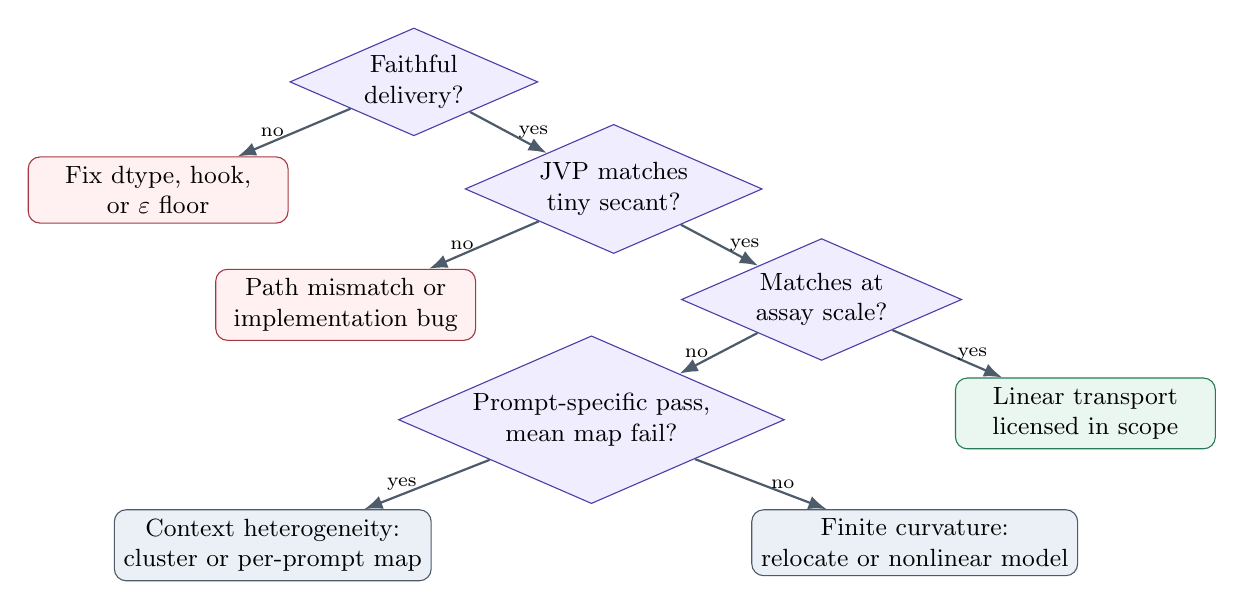
\begin{tikzpicture}[
  node distance=6mm and 8mm,
  q/.style={diamond,draw=violetdark,fill=lavender,aspect=2.3,align=center,font=\small,inner sep=1.5pt},
  a/.style={rectangle,rounded corners=1.5mm,draw=slate,fill=bluegray,align=center,font=\small,minimum width=33mm,minimum height=8mm},
  good/.style={rectangle,rounded corners=1.5mm,draw=greenish,fill=greenbg,align=center,font=\small,minimum width=33mm,minimum height=8mm},
  bad/.style={rectangle,rounded corners=1.5mm,draw=redish,fill=redbg,align=center,font=\small,minimum width=33mm,minimum height=8mm},
  arr/.style={-Latex,thick,draw=slate}
]
\node[q] (delivery) {Faithful\\delivery?};
\node[bad,below left=of delivery] (num) {Fix dtype, hook,\\or $\eps$ floor};
\node[q,below right=of delivery] (tiny) {JVP matches\\tiny secant?};
\node[bad,below left=of tiny] (bug) {Path mismatch or\\implementation bug};
\node[q,below right=of tiny] (finite) {Matches at\\assay scale?};
\node[q,below left=of finite] (context) {Prompt-specific pass,\\mean map fail?};
\node[good,below right=of finite] (pass) {Linear transport\\licensed in scope};
\node[a,below left=of context] (hetero) {Context heterogeneity:\\cluster or per-prompt map};
\node[a,below right=of context] (curve) {Finite curvature:\\relocate or nonlinear model};
\draw[arr] (delivery)-- node[left,font=\scriptsize] {no} (num);
\draw[arr] (delivery)-- node[right,font=\scriptsize] {yes} (tiny);
\draw[arr] (tiny)-- node[left,font=\scriptsize] {no} (bug);
\draw[arr] (tiny)-- node[right,font=\scriptsize] {yes} (finite);
\draw[arr] (finite)-- node[left,font=\scriptsize] {no} (context);
\draw[arr] (finite)-- node[right,font=\scriptsize] {yes} (pass);
\draw[arr] (context)-- node[left,font=\scriptsize] {yes} (hetero);
\draw[arr] (context)-- node[right,font=\scriptsize] {no} (curve);
\end{tikzpicture}
\caption{A decision tree for separating numerical failure, true curvature, and context-dependent tangent cancellation.}
\label{fig:decision_tree}
\end{figure}

\subsection{Thresholds should be control-calibrated}
There is no universal theorem that cosine 0.9 is sufficient or additivity error 0.2 is safe. Set acceptance regions relative to:
\begin{itemize}
  \item a positive-control model where the downstream assay is known to work;
  \item random and intervention-relevant directions;
  \item the exact behavioral dose used later;
  \item the stability needed for the intended claim.
\end{itemize}
Pre-register thresholds before inspecting the target model's behavioral outcomes.

\section{A formal answer to each question in the exchange}

\subsection{Why assume a linear map between arbitrary layers?}
One should not assume global linearity. The defensible assumption is local and empirical: around the model's typical states, and along the perturbation directions used by the assay, the first Taylor term may dominate over a useful radius. Residual paths, smooth activations, and stable attention routes can make that radius large, but do not guarantee it.

\subsection{Is local linearity needed for backpropagation?}
Only infinitesimal differentiability is needed to compute a gradient. Practical optimization benefits from a locally predictive gradient in parameter space, but recomputes after every update. The J-lens demands a finite activation-space approximation that remains useful across prompts. That is a much stronger requirement.

\subsection{Are we sure the Gemma result is real?}
The evidence is strong but not final. The corrected scale trend, faithful input delivery, OLMo positive control, superposition failure, and cross-corpus instability jointly make a real geometry difference plausible. The exact-JVP validation has now run (\cref{sec:autopsy-ran}): it \emph{operationally} reproduces the mismatch at every tested layer with the OLMo control passing under identical frozen gates --- and then quarantines itself behind a failed cross-backend parity ceiling. So the honest answer is unchanged in direction and sharpened in form: very probably real, still not licensed as a closed mechanism result, and now blocked on backend consistency rather than on missing evidence.

\subsection{Can we infer the cause without training scripts?}
Yes, at the mechanism level. Layerwise hooks, sublayer decomposition, frozen routing, norm linearization, JVPs, and context clustering can identify whether the culprit is attention routing, normalization, MLP gating, a late basis conversion, or mean-map cancellation. Training logs would be needed to explain why optimization selected this regime, not to localize the current forward-pass mechanism.

\subsection{Does it matter?}
Yes, in three ways:
\begin{enumerate}
  \item It defines an applicability boundary for a new interpretability method.
  \item It prevents a cross-model null from being mistaken for absence of a workspace.
  \item It warns that linear probes, steering vectors, and averaged attribution maps inherit checkpoint-specific geometry assumptions.
\end{enumerate}

\subsection{Can a nonlinear J-transform be reconstructed?}
For \emph{readout}, probably: an MLP probe, mixture of linear charts, or path-integrated Jacobian can model a nonlinear mapping. For \emph{causal ablation}, the problem is much harder. A fixed token direction and orthogonal projection are no longer globally well-defined; interventions become path- and context-dependent, and matched geometric controls lose their clean interpretation.

\section{Course exercises}

\subsection*{Exercise 1: Taylor scaling}
Let $F$ be $C^3$. Derive the leading-order scaling of:
\begin{enumerate}[label=(\alph*)]
  \item $\Delta(2\eps;v)-2\Delta(\eps;v)$;
  \item $\Delta(\eps;v)+\Delta(-\eps;v)$;
  \item $\Delta(\eps;v+w)-\Delta(\eps;v)-\Delta(\eps;w)$.
\end{enumerate}
Identify which Hessian contractions each expression estimates.

\subsection*{Exercise 2: RMSNorm geometry}
Derive \cref{eq:rmsnorm_jac}. Show that when $u$ is orthogonal to $h$, the second term vanishes. Interpret the result for perturbations tangent to a constant-norm sphere versus radial perturbations.

\subsection*{Exercise 3: softcap audit}
For $s_c(z)=c\tanh(z/c)$:
\begin{enumerate}[label=(\alph*)]
  \item prove that token rank is preserved;
  \item compute $s'_c(z)$ and $s''_c(z)$;
  \item explain why a post-unembedding softcap can create logit-space curvature without creating residual-to-residual curvature.
\end{enumerate}

\subsection*{Exercise 4: curvature versus context heterogeneity}
Assume
\[
  \Delta_x(\eps v)=\eps J_xv+\frac{1}{2}\eps^2H_x[v,v]+\cO(\eps^3).
\]
Design an estimator using at least three $\eps$ values that separates a nonzero relative-error floor from a term growing linearly with $\eps$. State the assumptions needed for identification.

\subsection*{Exercise 5: routing localization}
Gemma 4 31B repeats five sliding-attention layers and one full-attention layer. Specify a statistical test for whether nonlinear transport error is concentrated at full-attention blocks. Include the unit of resampling and a matched comparison that accounts for depth.

\subsection*{Exercise 6: nonlinear probe versus causal feature}
Construct a two-variable toy model in which a nonlinear probe decodes a label perfectly from $h$, but intervening to suppress the probe output does not change the model's final prediction. Explain which causal assumption fails.

\section{Solution sketches}

\subsection*{Exercise 1}
Using
\[
\Delta(\eps;v)=\eps Jv+\tfrac12\eps^2H[v,v]+\tfrac16\eps^3T[v,v,v]+\cdots,
\]
one obtains:
\begin{align*}
\Delta(2\eps;v)-2\Delta(\eps;v)
  &=\eps^2H[v,v]+\eps^3T[v,v,v]+\cO(\eps^4),\\
\Delta(\eps;v)+\Delta(-\eps;v)
  &=\eps^2H[v,v]+\cO(\eps^4),\\
\Delta(\eps;v+w)-\Delta(\eps;v)-\Delta(\eps;w)
  &=\eps^2H[v,w]+\cO(\eps^3).
\end{align*}

\subsection*{Exercise 2}
Differentiate $N(h)=\gamma\odot h/r(h)$ and use
\[
  Dr(h)[u]=\frac{\ip{h}{u}}{d\,r(h)}.
\]
If $u\perp h$, RMSNorm locally scales $u$ by $\gamma/r$ without the rank-one radial correction. Radial perturbations change the denominator and therefore experience stronger nonlinear gain effects.

\subsection*{Exercise 3}
Since $\tanh$ is strictly increasing, $z_i>z_j$ iff $s_c(z_i)>s_c(z_j)$. Also
\[
  s'_c(z)=\operatorname{sech}^2(z/c),
  \qquad
  s''_c(z)=-\frac{2}{c}\operatorname{sech}^2(z/c)\tanh(z/c).
\]
The softcap operates after residual transport and unembedding, so it cannot alter the hidden-state map measured before that point.

\subsection*{Exercise 4}
Estimate relative tangent error across scales and fit
\[
  e_{\mathrm{rel}}(\eps)\approx a+b\eps.
\]
A persistent $a>0$ suggests context mismatch or measurement bias; $b>0$ suggests smooth curvature. Identification requires faithful perturbation delivery, a reliable JVP, and an $\eps$ range small enough that higher orders do not dominate.

\subsection*{Exercise 5}
For each prompt, direction, and source layer, compute the increment in error across every downstream block. Compare full-attention increments with sliding-attention increments at matched relative depths, using prompt-family clustered bootstrap or a mixed model with prompt and source-direction effects. Pre-register the block labels and avoid selecting only visually large spikes.

\subsection*{Exercise 6}
Let the model output depend only on $a$, while $b=a^2$ is carried as a redundant correlate. A nonlinear probe can decode $a$ from $b$ up to sign if the data restricts $a\ge0$, yet changing $b$ while holding $a$ fixed leaves the output unchanged. Probe decodability does not identify the causal path.

\section{Suggested 90-minute lecture plan}

\begin{tabularx}{\textwidth}{@{}p{0.15\textwidth}X@{}}
\toprule
\textbf{Time} & \textbf{Activity}\\
\midrule
0--10 min & Present the Gemma rank cliff and ask students what it proves and what it does not.\\
10--25 min & Derive the prompt-specific Jacobian, corpus average, and J-lens readout. Emphasize affine versus linear transport.\\
25--40 min & Taylor remainder, finite-radius linearity, and the curvature/heterogeneity decomposition.\\
40--55 min & Derive RMSNorm and gated-MLP Jacobians; discuss attention routing.\\
55--68 min & Work through homogeneity, odd-symmetry, additivity, and exact JVP diagnostics.\\
68--78 min & Architecture autopsy of Gemma 4 31B, including the final-softcap correction.\\
78--87 min & Debate recovery options: late band, per-context maps, nonlinear probes, nonlinear causal removal.\\
87--90 min & Exit question: What claim is licensed today, and what single experiment most changes confidence?\\
\bottomrule
\end{tabularx}

\section{Summary}

\begin{takeawaybox}
\begin{enumerate}
  \item A deep transformer is globally nonlinear, but a trained residual network may still have a broad, useful local tangent regime.
  \item The J-lens needs more than differentiability: it needs finite-dose linearity and a stable mean Jacobian across contexts.
  \item Gemma 4 31B's middle band is output-opaque, and the supplied pilot reports finite-response and cross-context failures that make a fixed J-map doubtful there.
  \item The result does not imply that Gemma lacks intermediate concepts or a workspace. It implies that the current mid-band linear instrument is not licensed.
  \item Exact autograd JVPs, layerwise localization, and sublayer freezing can determine whether the dominant cause is curvature, routing, normalization, MLP gating, or context cancellation.
  \item Nonlinear probes may recover readout, but a clean nonlinear analogue of token-direction projection is a much harder causal problem.
  \item The practical methodological contribution is a transport gate: test the premise before interpreting a cross-model null.
\end{enumerate}
\end{takeawaybox}

\section*{References}
\addcontentsline{toc}{section}{References}
\small
\begin{thebibliography}{99}

\bibitem{gurnee2026}
W. Gurnee, N. Sofroniew, A. Pearce, M. Piotrowski, I. Kauvar, R. Chen, A. Soligo, P. Bogdan, E. Ong, R. Wang, B. Thompson, D. Abrahams, S. Kantamneni, E. Ameisen, J. Batson, and J. Lindsey.
\newblock Verbalizable representations form a global workspace in language models.
\newblock \emph{Transformer Circuits Thread}, 2026. arXiv:2607.15495.
\newblock \url{https://transformer-circuits.pub/2026/workspace/}

\bibitem{gemma4report}
Gemma Team, Google DeepMind.
\newblock Gemma 4 technical report.
\newblock arXiv:2607.02770, 2026.

\bibitem{gemma4config}
Google and Hugging Face.
\newblock Official \texttt{google/gemma-4-31B} configuration and Transformers implementation, accessed July 2026.
\newblock \url{https://huggingface.co/google/gemma-4-31B}

\bibitem{vaswani2017}
A. Vaswani et al.
\newblock Attention is all you need.
\newblock \emph{Advances in Neural Information Processing Systems}, 2017.

\bibitem{rmsnorm}
B. Zhang and R. Sennrich.
\newblock Root mean square layer normalization.
\newblock \emph{Advances in Neural Information Processing Systems}, 2019.

\bibitem{qknorm}
A. Henry, P. R. Dachapally, S. S. Pawar, and Y. Chen.
\newblock Query-key normalization for transformers.
\newblock \emph{Findings of EMNLP}, 2020.

\bibitem{tunedlens}
N. Belrose et al.
\newblock Eliciting latent predictions from transformers with the tuned lens.
\newblock arXiv:2303.08112, 2023.

\bibitem{gemma2code}
Google and Hugging Face.
\newblock Gemma 2 gated MLP and RMSNorm reference implementation.
\newblock \url{https://github.com/huggingface/transformers/tree/main/src/transformers/models/gemma2}

\bibitem{pilot}
K. Burtram.
\newblock \emph{J-space, Part 2: The Model Matrix}, living campaign handout and associated nonlinear-transport exchange.
\newblock Unpublished course and research materials, July 2026.

\end{thebibliography}

\end{document}
